% Source: graduate-coursework/Research/Intro_to_Agents/handouts/Part2_Agent_Foundations.tex

\documentclass[border=4pt]{standalone}
\usepackage{amsmath}
\usepackage{amssymb}
\usepackage{tikz}
\usepackage{xcolor}
\usetikzlibrary{shapes.geometric, arrows.meta, positioning, fit, calc, backgrounds}

\definecolor{UofSCGarnet}{HTML}{73000a}
\definecolor{UofSCBlack}{HTML}{000000}
\definecolor{UofSCWhite}{HTML}{ffffff}
\definecolor{UofSCAtlantic}{HTML}{466A9F}
\definecolor{UofSCCongaree}{HTML}{1F414D}
\definecolor{UofSCRose}{HTML}{CC2E40}
\definecolor{UofSCHorseshoe}{HTML}{65780B}
\definecolor{UofSCGrass}{HTML}{CED318}
\definecolor{UofSCHoneycomb}{HTML}{A49137}
\definecolor{UofSCDarkGarnet}{HTML}{570008}
\definecolor{UofSCAzalea}{HTML}{844247}
\definecolor{UofSC90Black}{HTML}{363636}
\definecolor{UofSC70Black}{HTML}{5C5C5C}
\definecolor{UofSC50Black}{HTML}{A2A2A2}
\definecolor{UofSCWarmGrey}{HTML}{676156}
\definecolor{UofSCSandstorm}{HTML}{FFF2E3}

\tikzset{
    % Box styles with sharp corners
    component/.style={
        rectangle,
        draw=UofSCBlack,
        fill=UofSCWhite,
        thick,
        minimum width=3cm,
        minimum height=1cm,
        align=center,
        font=\small
    },
    component garnet/.style={
        component,
        fill=UofSCGarnet!10,
        draw=UofSCGarnet,
        thick
    },
    component atlantic/.style={
        component,
        fill=UofSCAtlantic!10,
        draw=UofSCAtlantic,
        thick
    },
    component congaree/.style={
        component,
        fill=UofSCCongaree!10,
        draw=UofSCCongaree,
        thick
    },
    loop node/.style={
        rectangle,
        draw=UofSCGarnet,
        fill=UofSCGarnet!15,
        thick,
        minimum width=2.5cm,
        minimum height=1.2cm,
        align=center,
        font=\footnotesize\bfseries
    },
    decision/.style={
        diamond,
        draw=UofSCBlack,
        fill=UofSCHoneycomb!20,
        thick,
        minimum width=2cm,
        minimum height=1.5cm,
        align=center,
        font=\footnotesize,
        aspect=2
    },
    arrow style/.style={
        ->,
        >=Stealth,
        thick,
        UofSCBlack
    },
    biarrow style/.style={
        <->,
        >=Stealth,
        thick,
        UofSCBlack
    }
}

\begin{document}
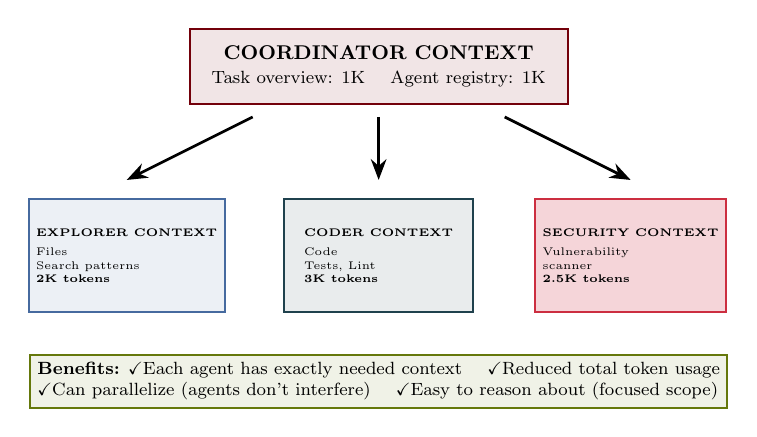
\begin{tikzpicture}[scale=0.8, transform shape]
        % Coordinator at top
        \node[component garnet, minimum width=6cm, minimum height=1.2cm] (coordinator) at (0, 3) {
            \textbf{COORDINATOR CONTEXT}\\
            \footnotesize Task overview: 1K \quad Agent registry: 1K
        };

        % Connection lines
        \draw[arrow style, line width=1pt] (-2, 2.2) -- (-4, 1.2);
        \draw[arrow style, line width=1pt] (0, 2.2) -- (0, 1.2);
        \draw[arrow style, line width=1pt] (2, 2.2) -- (4, 1.2);

        % Specialist agents
        \node[component atlantic, minimum width=3cm, minimum height=1.8cm, font=\tiny, align=left] (explorer) at (-4, 0) {
            \textbf{EXPLORER CONTEXT}\\[0.1cm]
            Files\\
            Search patterns\\
            \textbf{2K tokens}
        };

        \node[component congaree, minimum width=3cm, minimum height=1.8cm, font=\tiny, align=left] (coder) at (0, 0) {
            \textbf{CODER CONTEXT}\\[0.1cm]
            Code\\
            Tests, Lint\\
            \textbf{3K tokens}
        };

        \node[component, fill=UofSCRose!20, draw=UofSCRose, minimum width=3cm, minimum height=1.8cm, font=\tiny, align=left] (security) at (4, 0) {
            \textbf{SECURITY CONTEXT}\\[0.1cm]
            Vulnerability\\
            scanner\\
            \textbf{2.5K tokens}
        };

        % Benefits box
        \node[draw=UofSCHorseshoe, thick, fill=UofSCHorseshoe!10, minimum width=10cm, align=left, font=\footnotesize] (benefits) at (0, -2) {
            \textbf{Benefits:} \checkmark Each agent has exactly needed context \quad \checkmark Reduced total token usage\\
            \checkmark Can parallelize (agents don't interfere) \quad \checkmark Easy to reason about (focused scope)
        };
    \end{tikzpicture}
\end{document}
